
\begin{frame}[t]{Motivación del proyecto}

        \centering
        En el Laboratorio de Electrónica Cuántica (LEC) se dispone de un microscopio SPIM    
        \begin{figure}[H]
            \centering
            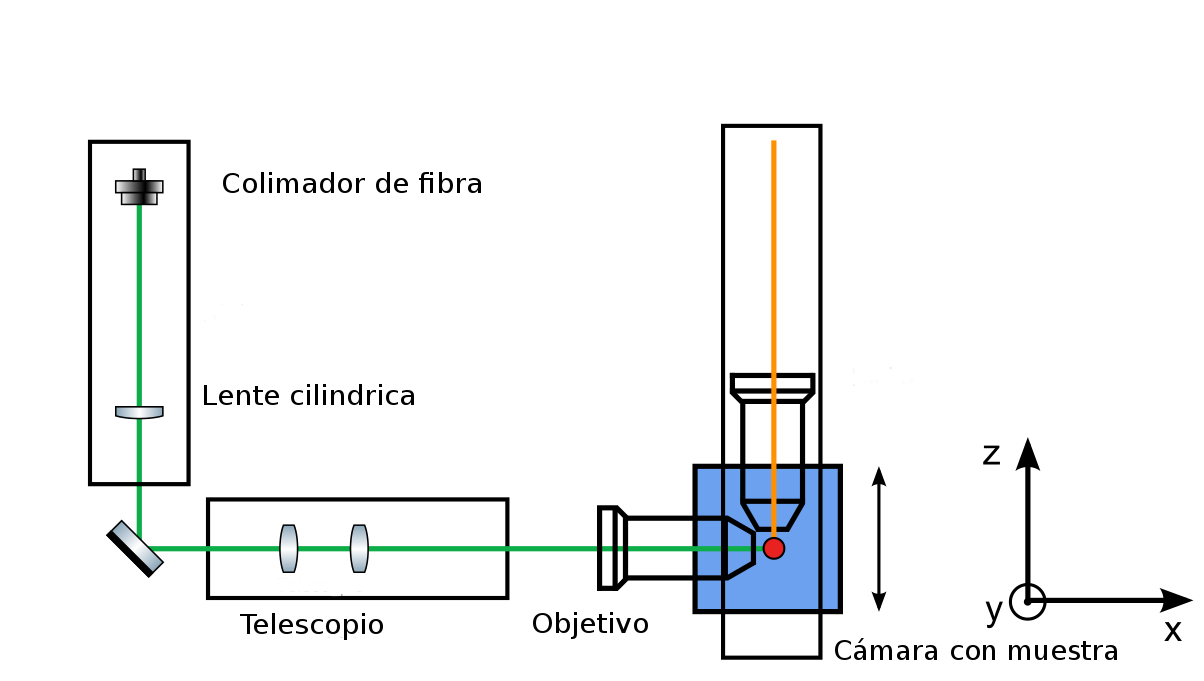
\includegraphics[width=0.8\textwidth]{fig/spim_anotado}
            \label{fig:spim} 
        \end{figure}
        
    \end{frame}
    
    \begin{frame}{Anisotropía de Fluorescencia}

    Anisotropía: cambio de la polarización de luz de fluorecencia, al iluminar con luz linealmente polarizada

    \begin{figure}
        \centering
        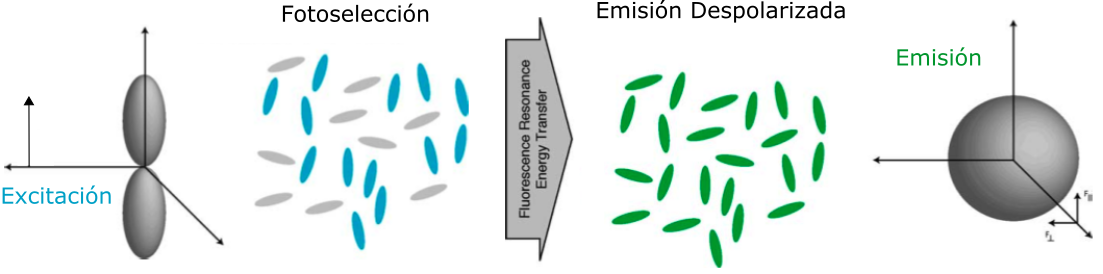
\includegraphics[width=1\textwidth]{fig/fotoseleccion.png}
    \end{figure}
    
   \end{frame}  
    
    %\ImagenCitada{\tiny{Adaptado de \titulopaper{HomoFRET Fluorescence Anisotropy Imaging as a Tool to Study Molecular Self-Assembly in Live Cells}, \autorpaper{Chan et al.}, \revistapaper{ChemPhysChem}}}
    
\begin{frame}{Mediciones del SPIM}
    \centering
    En este microscopio requiere determinar       
        \begin{figure}[H]
            \centering
            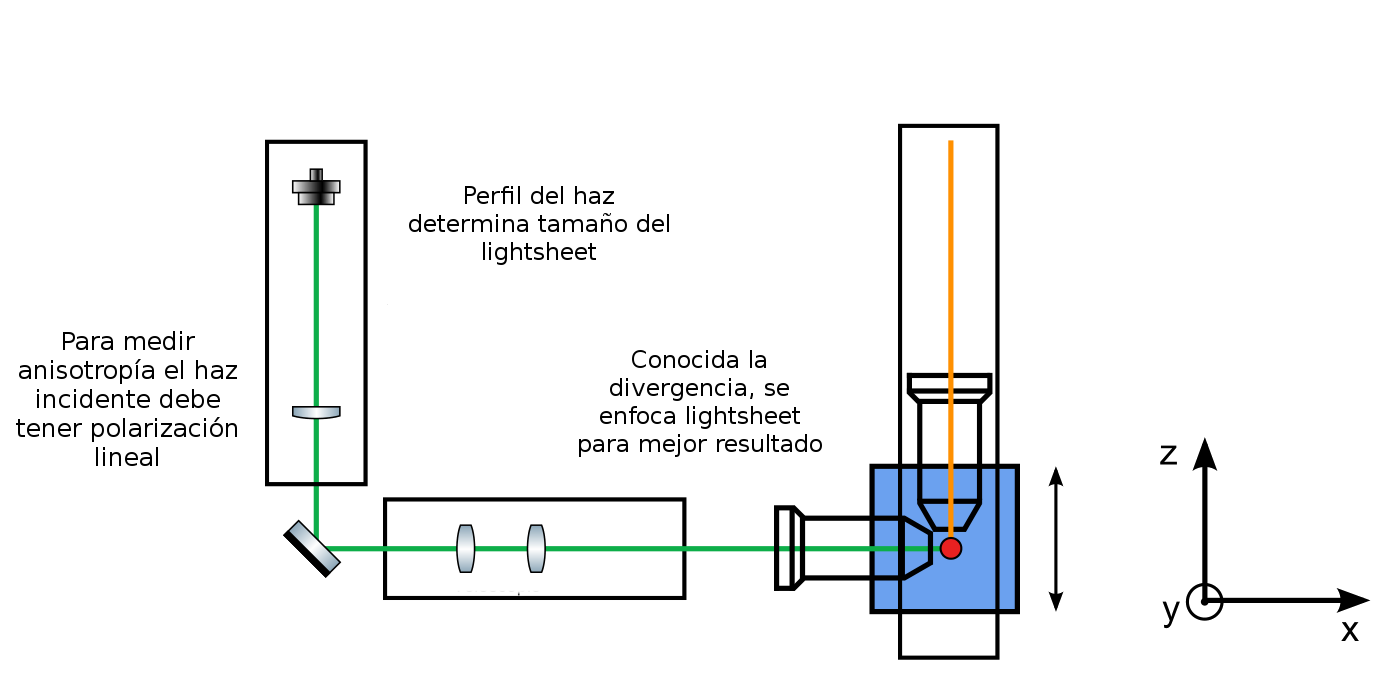
\includegraphics[width=0.9\textwidth]{fig/spim_mediciones}
            \label{fig:spim} 
        \end{figure}
\end{frame}

